In this section there is a complete view of hot the web application is going to look. 
It includes diagrams that show hot the users can navigate in the user interfaces offered by the aplication.
Its main purpose is to describe in details the mockups that are already presented in the RASD (reference). Therefore it is easier to understand 
the main features that the system offers.


\subsection{UX diagrams}
This subsection focuses on the flow of the windows of the web application, 
both for farmers and policy makers.

\begin{figure}[H]
    \begin{center}
          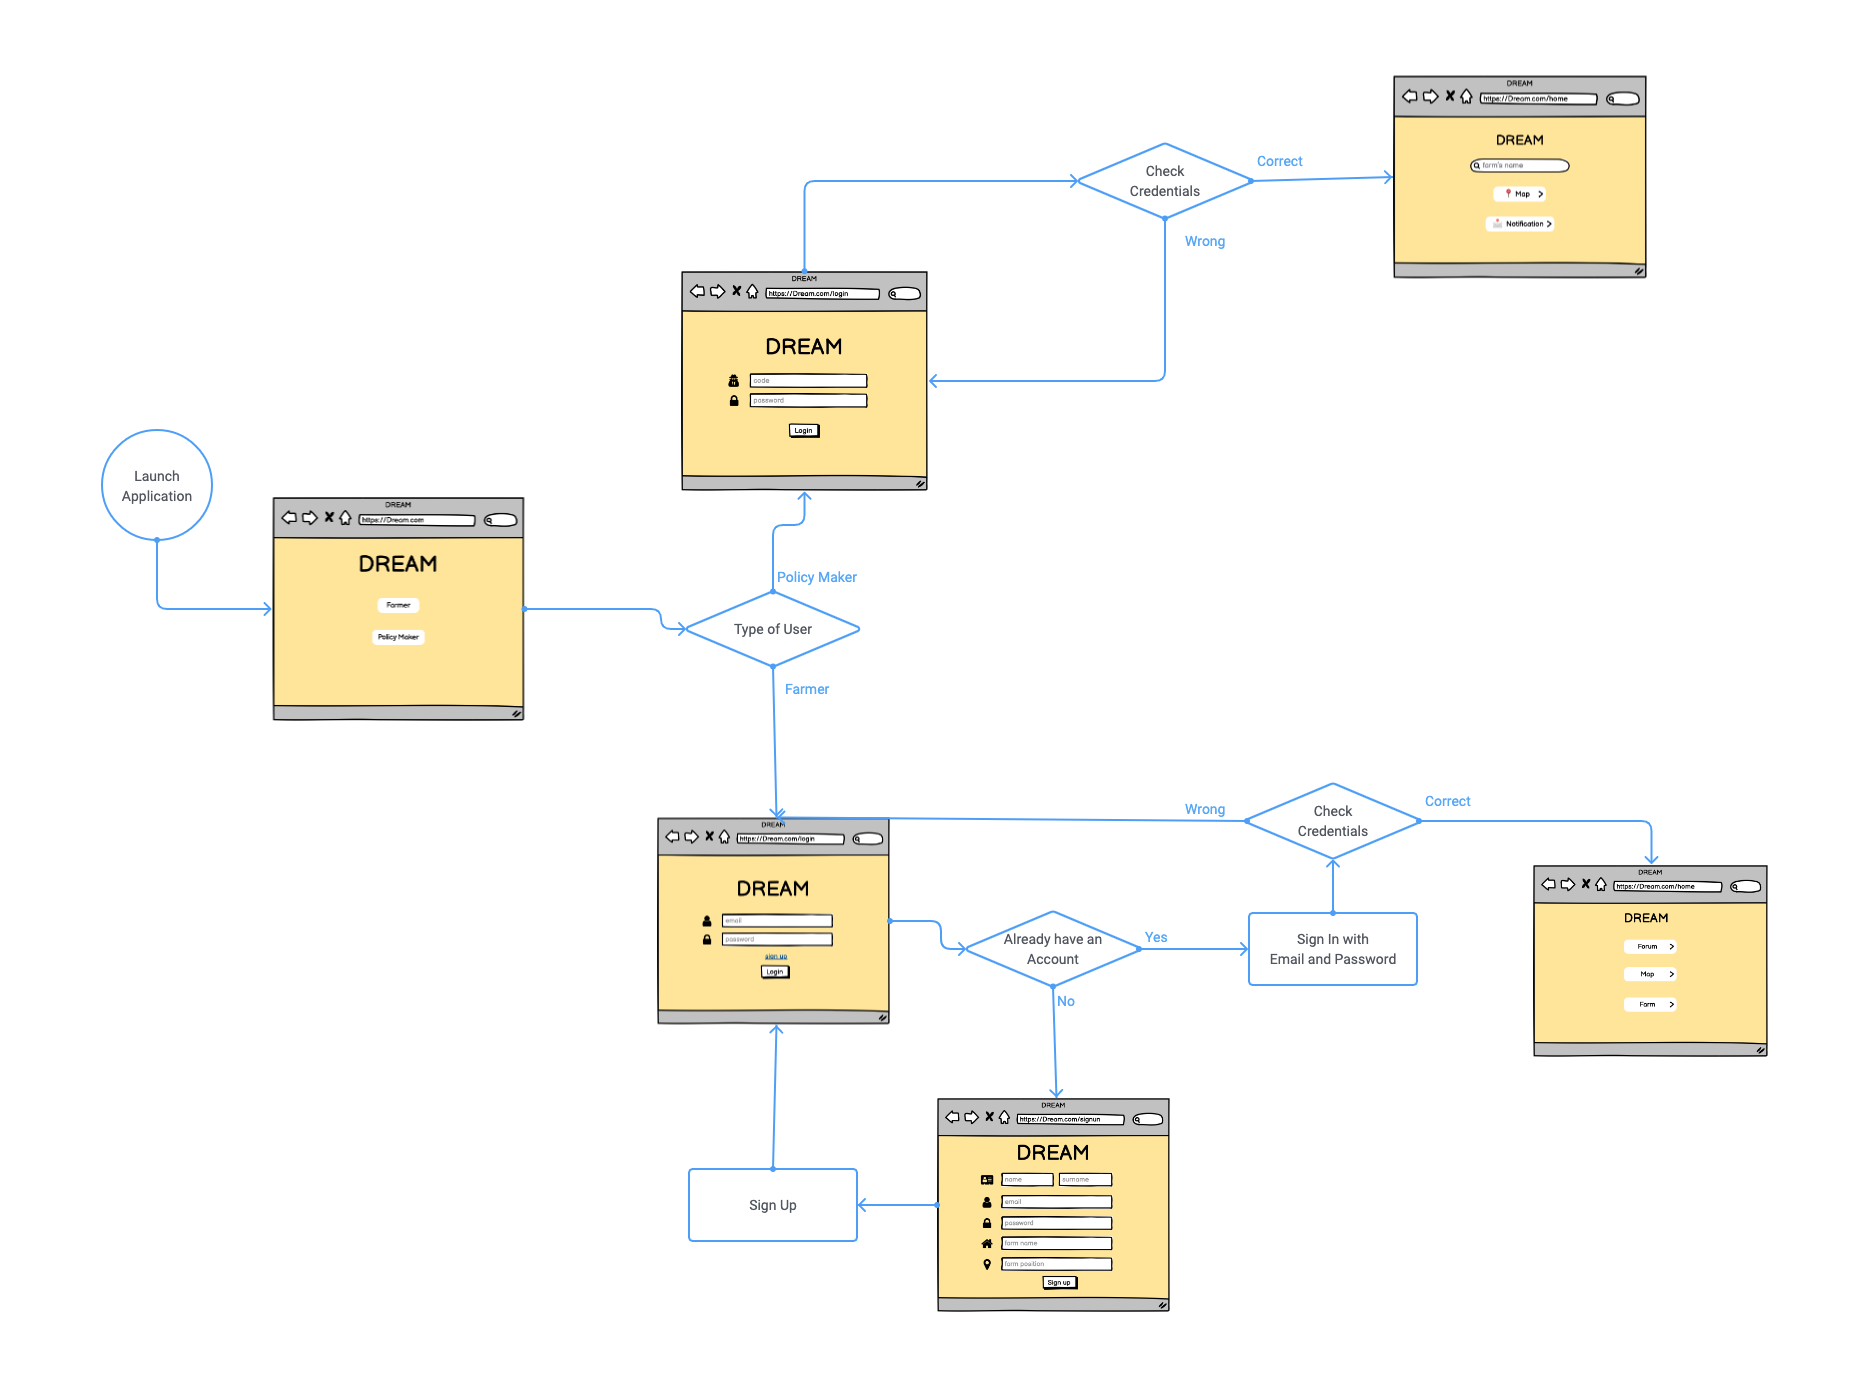
\includegraphics[width=1\textwidth]{images/UXdiagram_login.png}
          \caption{Sign Up \& Sign In}
    \end{center}
\end{figure}

\begin{figure}[H]
    \begin{center}
          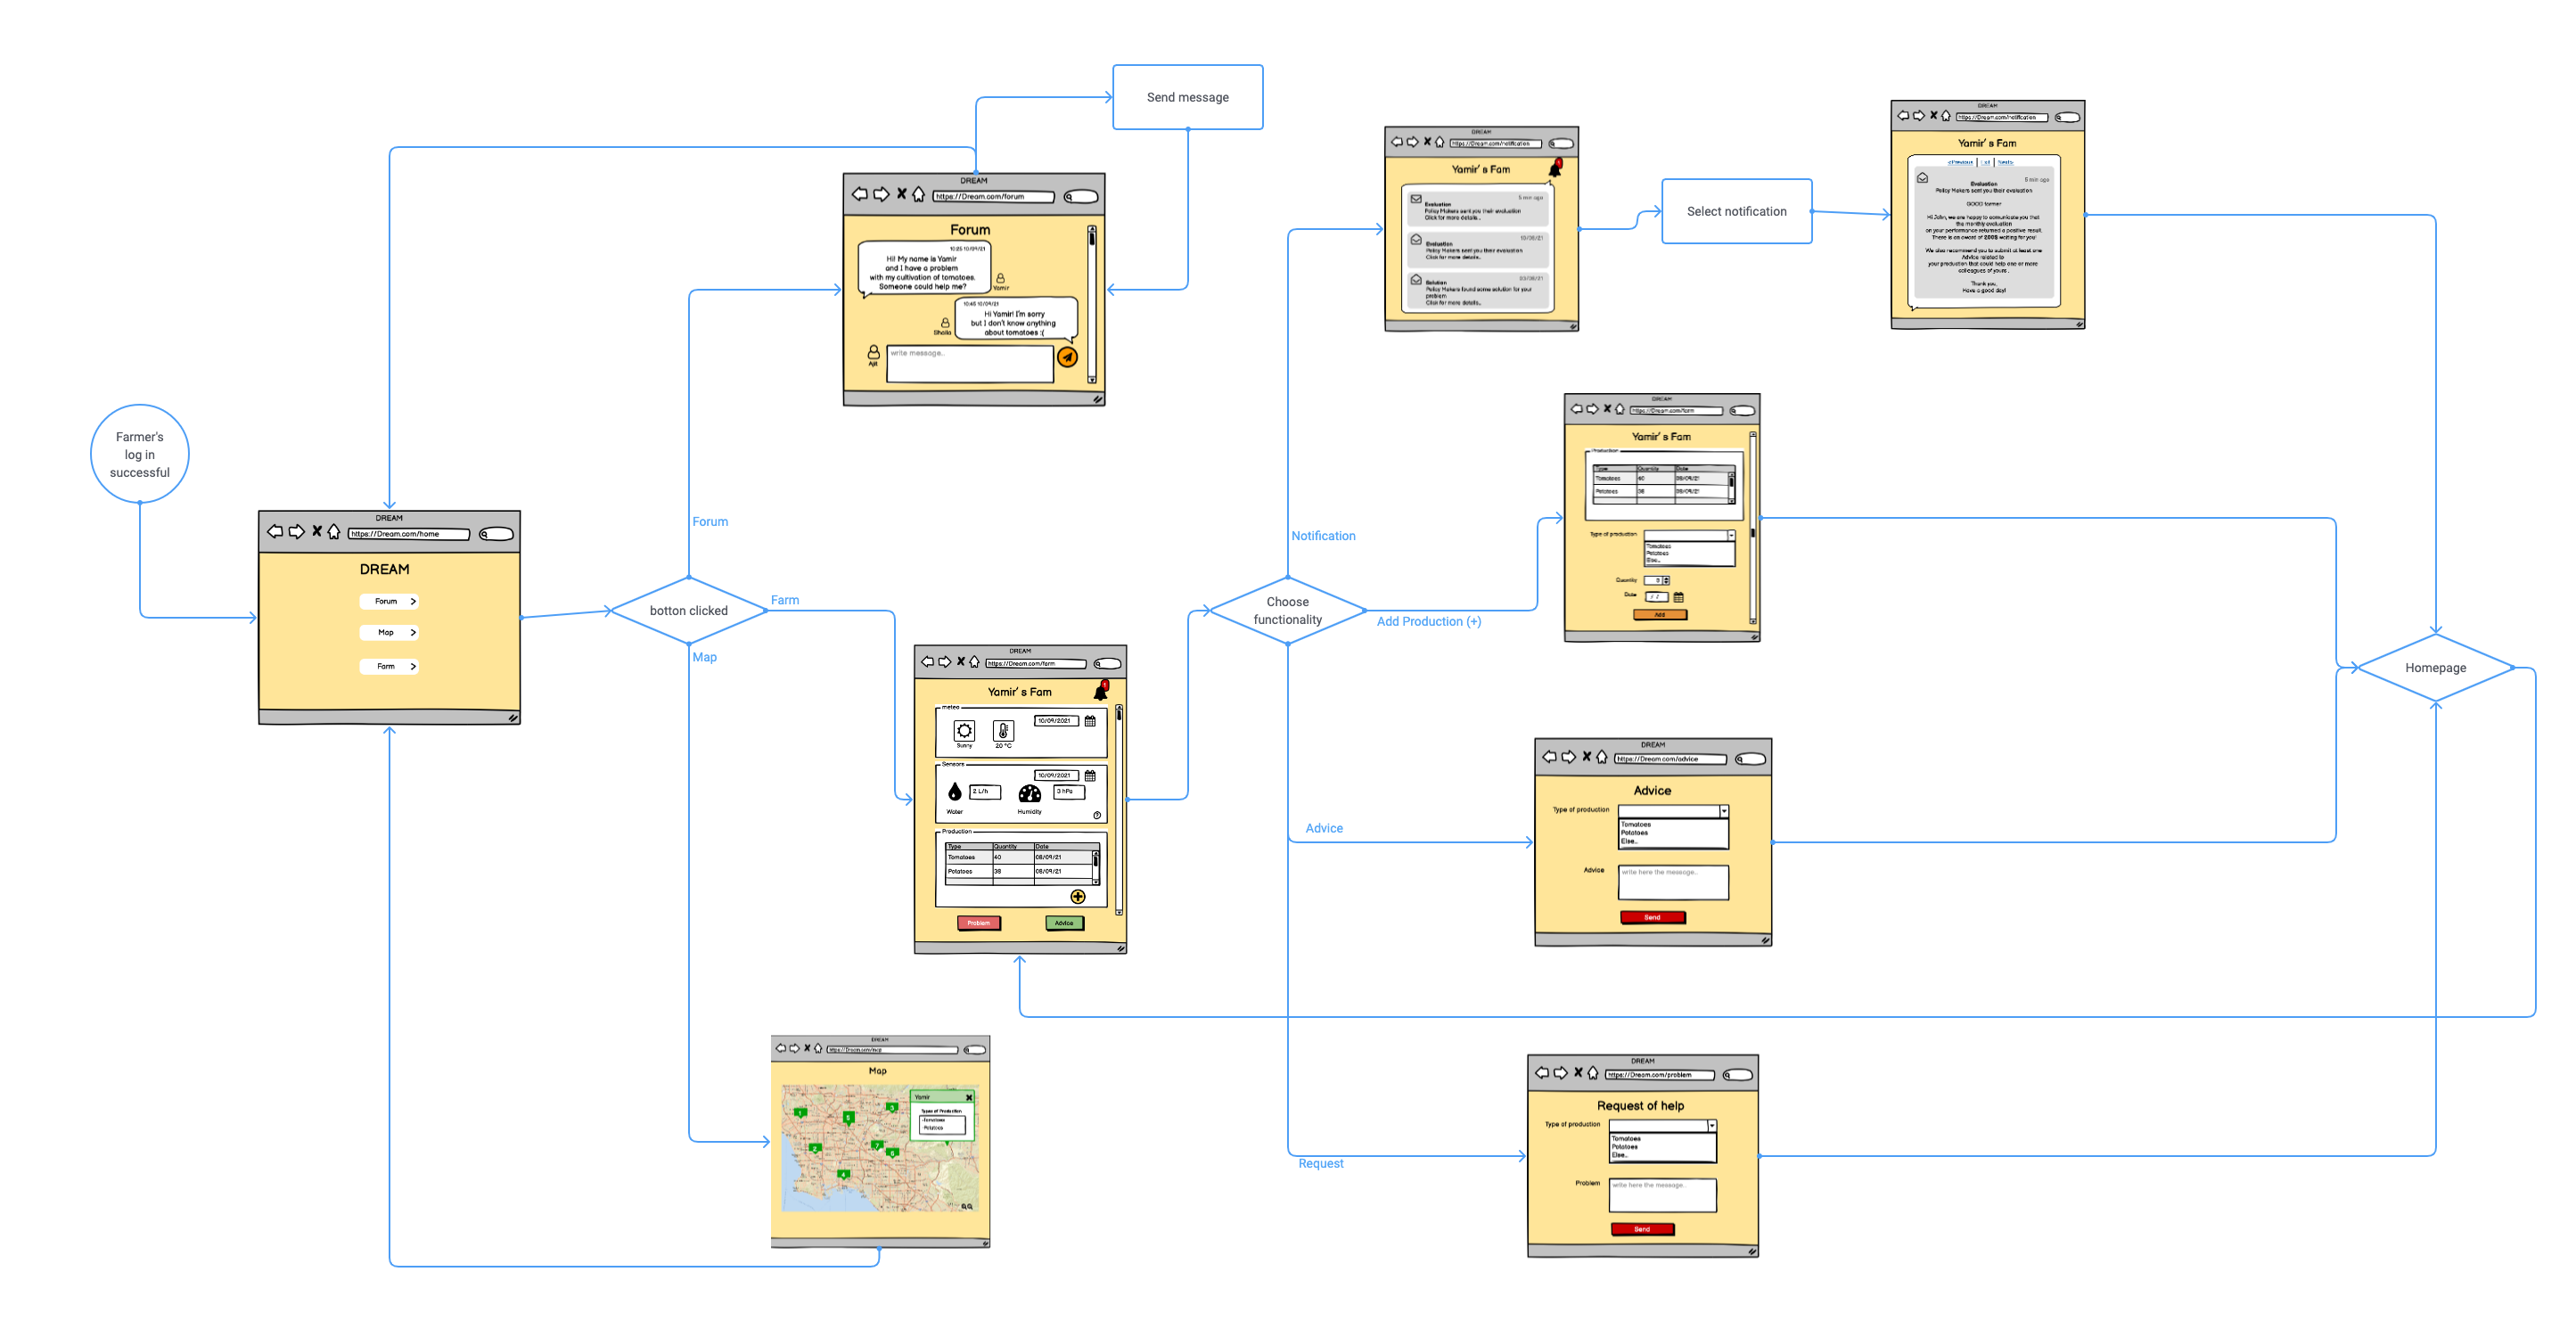
\includegraphics[width=1\textwidth]{images/UXdiagram_farmer.png}
          \caption{Farmer Web Application}
    \end{center}
\end{figure}
\begin{figure}[H]
    \begin{center}
          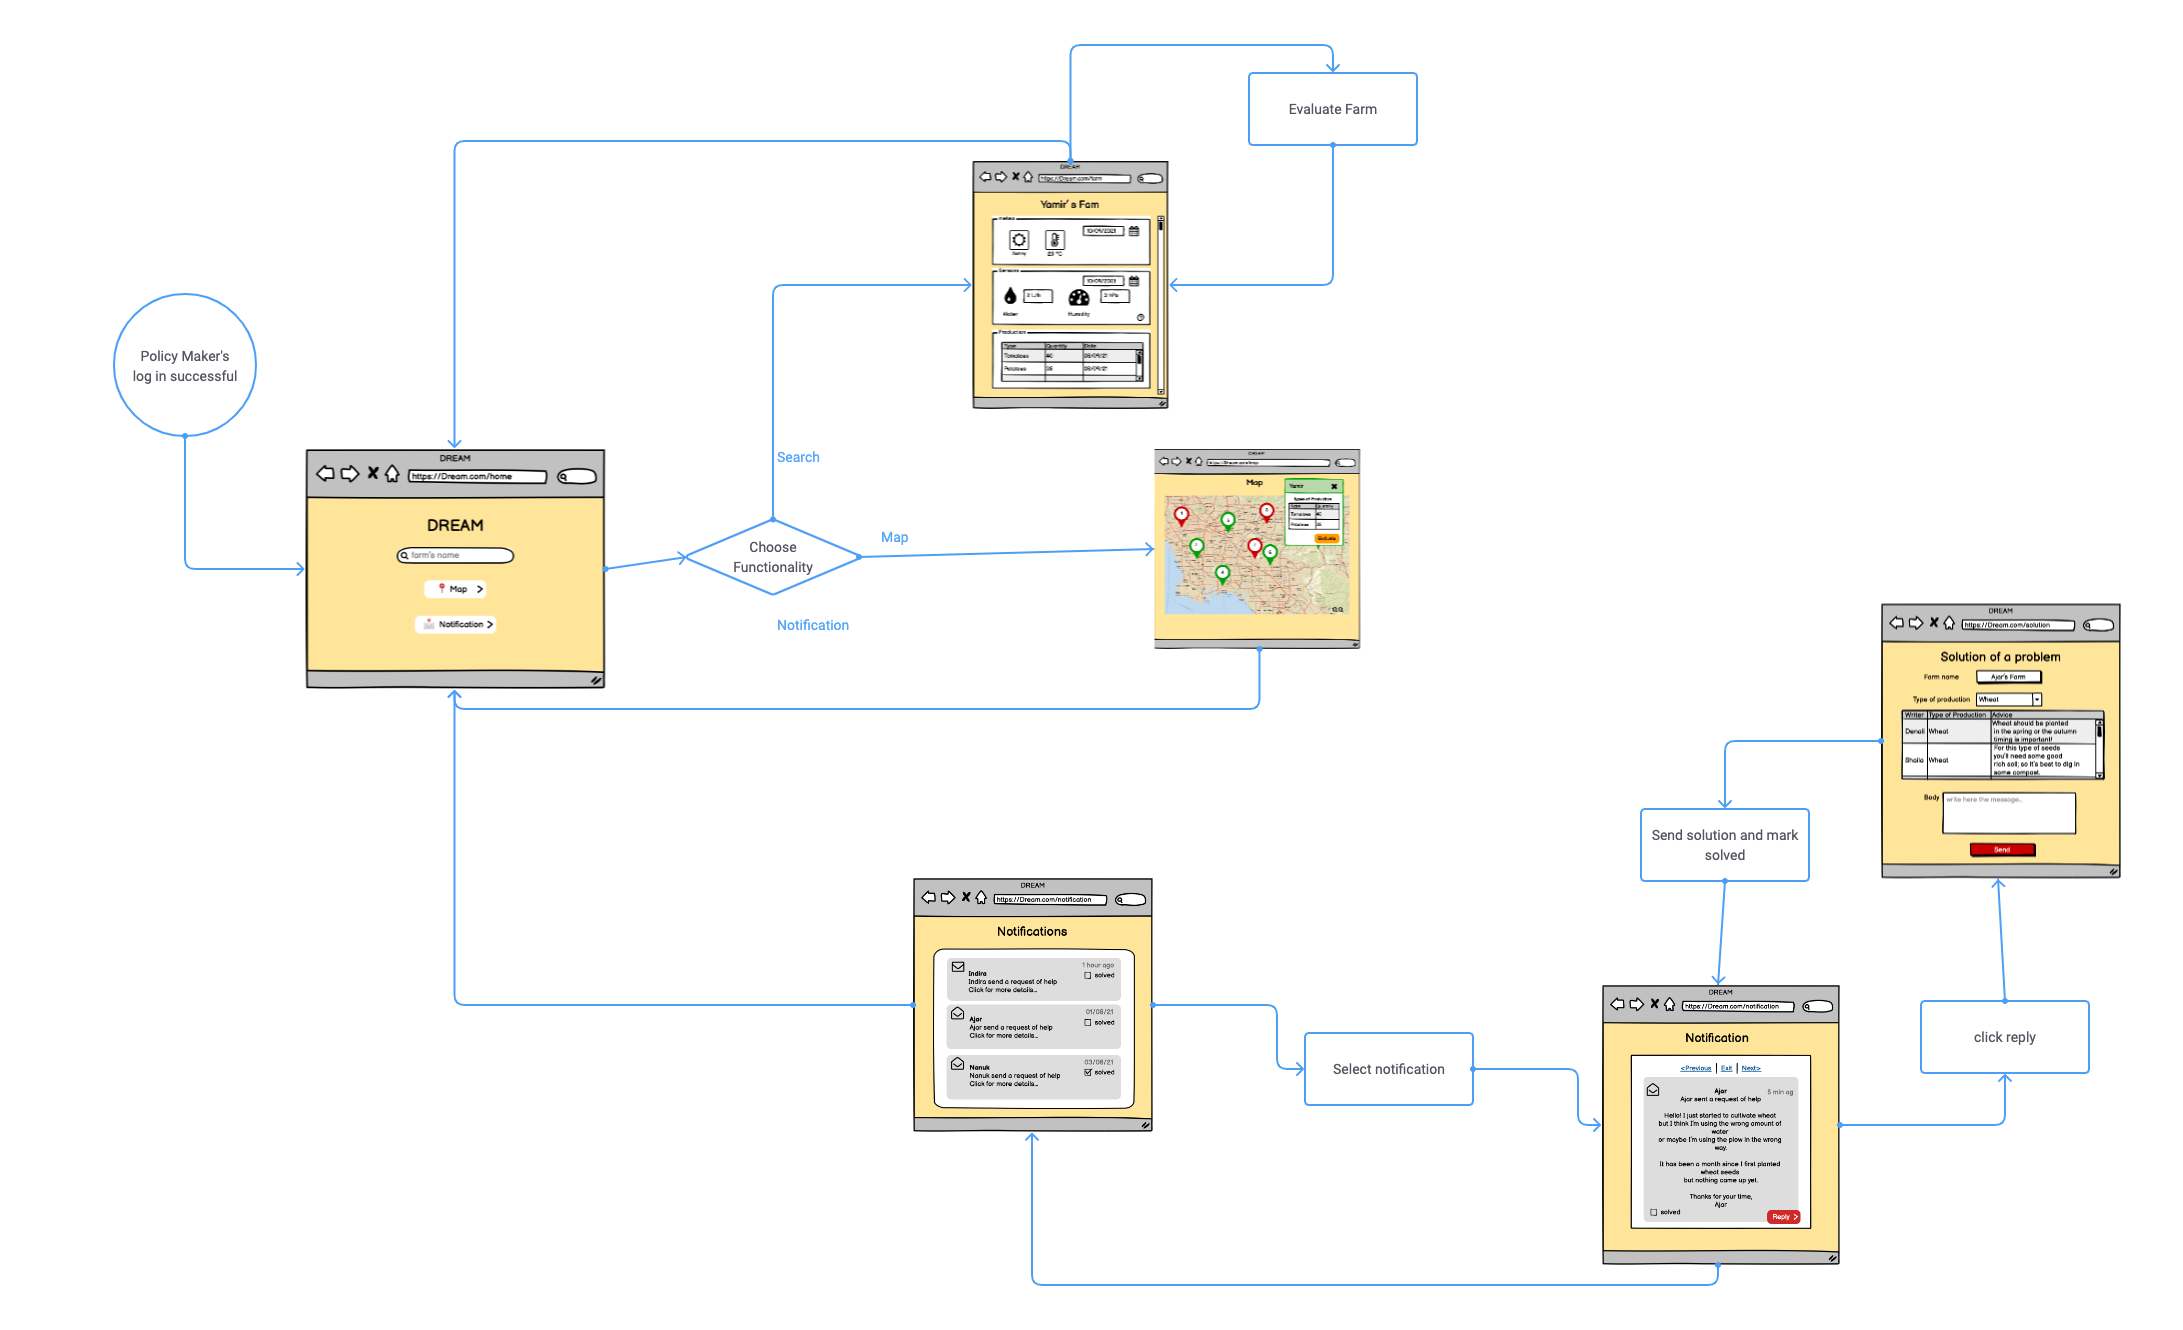
\includegraphics[width=1\textwidth]{images/UXdiagram_policymaker.png}
          \caption{Policy Maker Web Application}
    \end{center}
\end{figure}

\subsection{Web application}
\textbf{Dream's homepage} \\
The first mockup (Figure ..) is the first page that every user sees when accessing the web application. 
A user can click the button of the type of user that characterizes him.

\subsubsection{Farmer Web Application}
\textbf{Login}\\ 
The mockup showed in Figure .. is the initial page that every farmer sees after selecting the type of user. A  farmer can interact with the application only 
after being authenticated. Therefore the farmer can decide to sign up if it is the first time ever that he uses the application or to login in through his authenticated credentials.
In order to login the user has to provide its email and his password. After being recognized he will be redirected to the home page which is going to be described in the next paragraphs.

\textbf{Registration} \\
The mockup showed in Figure .. is the sign up page, it allows the farmer to create a new account. This allows him to provide first the information related to his new account. 
Therefore he need to write his personal information: name, surname, email and password and in addition to that he must insert his farm name and position.
The sign up button will add the new farmer to the system and redirect the user to the login page where he can access the system.

\textbf{Homepage}\\
The homepage of the farmer's web application allows the user to select the features offered by the system:
\begin{itemize}
    \item Forum
    \item Map
    \item Farm
\end{itemize}
After clicking one of this buttons the farmer will be redirected to the selected pages, which are goin to be described in the next paragraphs.

\textbf{Forum}\\
The mockup in Figure .. shows a basic example of what the forum page will look like. The farmer on this page is able to read messages written by other farmer or 
write a message in order to answer or ask something to the other ones. After he types a message he need to click send in order to add the message in the application. 
After the button is clicked the user can see an updated version of this page.

\textbf{Map}\\
After selecting the map functionality on the homepage the user can see an updated version of the map, 
an example of it is showed in Figure ... The farmer on this page can see the location and name of the other farms and see what type of production 
they have.


\textbf{Farm Page}\\ 


\textbf{Send Advice}\\


\textbf{View Notification}\\


\textbf{Send Request}\\


\textbf{Add Production Data}\\


\subsubsection{Policy Maker Web Application}
\textbf{Login} \\
The mockup showed in Figure .. is the initial page that every policy maker sees after selecting the type of user.
A policy maker can interact with the system only after being authenticated. Therefore the policy maker needs to own the authentication code and password previously given to him.
Once being recognized the application will redirect him to the home page which is going to be described in the next paragraphs.